\subsection{Fundamental Particles and Interactions}
\label{sec:Intro_FundParticles}

The SM describes interactions of elementary particles. There are four fundamental interactions: electromagnetic, strong, weak and gravitational. The gravity is not included into the SM but its effect on particles is negligible compared to the other forces which makes it possible to develop a theory of the particle physics and conduct experiments even without having the gravity included into the model.\\ 

All fundamental elementary particles in the SM can be split into three categories by their spins. There are fermions which possess spin s=1/2, there are gauge bosons which are vector particles (s=1) and there is the Higgs boson which is a scalar particle (s=0). \\

The fermions are arranged into three generations, each generation consists of a quark with charge Q=$+$2/3(up, charm, and top quarks), a quark with Q=$-$1/3 (down, strange, and bottom quarks), a charged lepton with Q=$-$1 (electron, muon, and tau-lepton) and a neutrino (electron, muon, and tau neutrinos) which is electrically neutral. Each quark can carry any of three colors: red, blue, or green. Additionally, each fermion has its antiparticle. Therefore, the total number of fundamental fermions is $(6 ($leptons$)+6 ($quarks$) \cdot 3 ($colors$) ) \cdot 2 ($to~include~antiparticles$) = 48$.\\ 

Corresponding particles in different generations have the same charges, spins and interaction properties but masses of particles increase with a generation. These mass differences lead to different decay properties because a particle A can decay to particles B and C only if their masses relate as $m_A > m_B + m_C$. Thus, an electron is a stable particle, a muon decays as $\mu^- \rightarrow e^- + \bar{\nu_e} + \nu_\mu$, a tau-lepton, as the heaviest charged lepton, has the largest number of decay channels amongst the charged leptons: $\tau^- \rightarrow \mu^- + \bar{\nu_\mu} + \nu_\tau$, $\tau^- \rightarrow e^- + \bar{\nu_e} + \nu_\tau$,  $\tau^- \rightarrow \nu_\tau +$ quarks. \\

In addition to fermions, the SM includes gauge bosons which are interaction mediators. They are called mediators because fermions interact with each other by exchanging them. For example, two charged fermions can interact with each other by exchanging a photon. Such interaction is called electromagnetic interaction and a photon is a mediator for the electromagnetic interaction. Similarly, a gluon is a mediator for strong interactions, and W$^{\pm}$ and Z$^0$ bosons are mediators for weak interactions. W$^{\pm}$ and Z$^0$ bosons are massive while a photon and a gluon are massless particles. \\

The last SM particle is the Higgs boson. The Higgs boson is a scalar neutral particle which is playing a critical role in the electroweak symmetry breaking. The Higgs mechanism explains how $W$ and $Z$ bosons become massive particles.\\

All the particles are summarized in Fig.~\ref{fig:SMtable}. These and only these fundamental particles and their antiparticles have been discovered by now. However, there are many composite particles which are called hadrons. Hadrons can consist of three quarks (baryons), quark and antiquark (meson), or three antiquarks (antibaryons). Hadrons always possess an integer charge.\\

Most of the particles are short-lived and decay within microseconds. The only stable particles are protons and antiprotons, electrons and positrons, neutrinos and antineutrinos, photons, and, in some sense, gluons. However, if a particle cannot decay, it does not mean that it would live forever. There are many different kinds of reactions in which particles can disappear. Antiprotons and positrons would immediately annihilate with protons and electrons, photons can be absorbed by charged particles, electrons and protons can scatter to produce neutrons and neutrinos and many other reactions are possible.\\ 

In this dissertation, the study of $pp\rightarrow W\gamma + X$ process where the $W$ decays as $W\to \ell\nu$ where $\ell = e, \mu$ is reported. The $W\gamma$ production with leptonic $W$ decays proceeds through one of the following three processes: the initial state radiation where a photon is emitted from one of the incoming partons, the final state radiation where a photon is radiated off the charged lepton from the $W$ boson decay, and, finally, the triple gauge coupling (TGC) where a photon is emitted from the $W$ boson. Many BSM theories predict an enchancement of the TGC production over the SM value and, therefore, the experimental search for such an enchancement is a good test for such theories.\\ 
%The total and the differential cross section with respect to the photon transverse momentum ($P_T^\gamma$) has been measured. The $P_T^{\gamma}$ is sensitive to the potential anomalous TGC (aTGC) in the high $P_T^{\gamma}$ region. The disagreement between the measured and theoretically predicted differential cross section at the higher $P_T^{\gamma}$ end would be an indication of the possible presence of the aTGC.

%In this dissertation a process is studied where quark and antiquark interact to produce a $W$ boson which then decay as $W^\pm \rightarrow e^\pm \nu_e(\bar{\nu_e})$ or $W^\pm \rightarrow \mu^\pm \nu_\mu(\bar{\nu_\mu}) $. A photon is radiated off a quark or antiquark, a charged lepton or a $W$ boson. The most interesting mechanism out of three is a radiation from a $W$ boson because this is the triple gauge coupling where we potentially can have a new physics. 

Therefore, the focus of this study is an interaction between a photon and a $W$ boson however many other SM particles are relevant too. Thus, a charged lepton and a neutrino appear as the final state particles, a quark and an antiquark appear as initial state particles and all fundamental particles except the Higgs boson participate in various background processes. Subsections \ref{sec:Intro_Electroweak}-\ref{sec:Intro_ppCollisions}, chapter \ref{sec:WgAbout} and \cite{ref_Griffiths} describe particle interactions in more details.\\


\begin{figure}[htb]
  \begin{center}
    {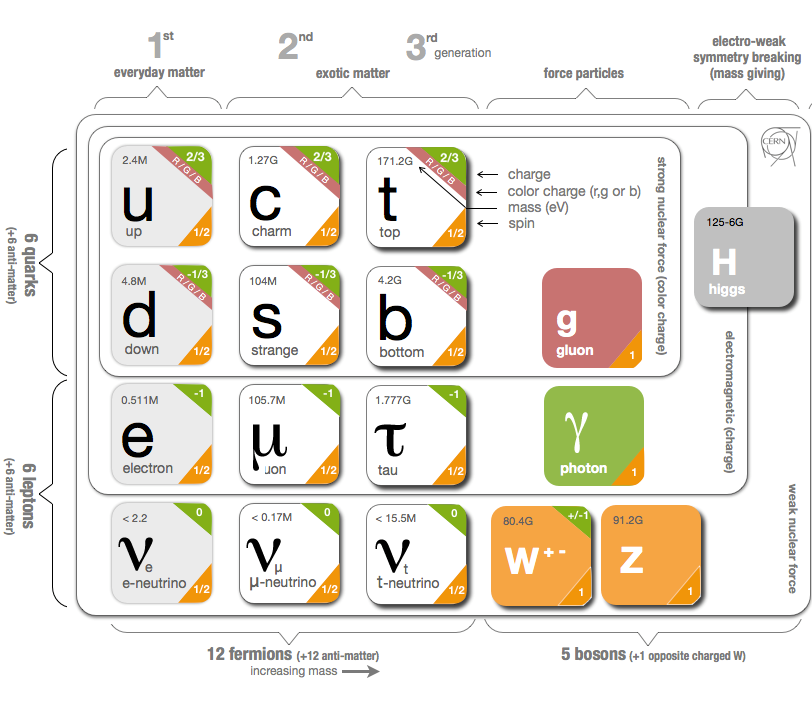
\includegraphics[width=0.90\textwidth]{../figs/Intro/StandardModel.png}}
    \caption{Standard Model Particles and Interations. Source of the figure: \cite{ref_fig_SM}.}
    \label{fig:SMtable}
  \end{center}
\end{figure}





